\documentclass[12pt, fullpage,letterpaper]{exam}

\usepackage[margin=1in]{geometry}
\usepackage{url}
\usepackage{amsmath,amsthm,amssymb}
\usepackage{graphics}
\usepackage{pgfplots}
\usepgfplotslibrary{polar}
\usepgflibrary{shapes.geometric}
\usetikzlibrary{calc}

\pgfplotsset{my style/.append style={axis x line=middle, axis y line=
middle, xlabel={$x$}, ylabel={$y$}, axis equal }}

\newcommand{\semester}{Fall 2015}
\newcommand{\assignmentId}{3}
\newcommand{\releaseDate}{Oct 20, 2015}
\newcommand{\dueDate}{Nov 3, 2015}

\newcommand{\bx}{{\bf x}}
\newcommand{\bw}{{\bf w}}

\title{CS 5350/6350: Machine Learning \semester}
\author{Homework \assignmentId}
\date{Handed out: \releaseDate\\
  Due date: \dueDate}
\printanswers
\begin{document}
\maketitle


\section{Warm Up: Feature Expansion}
\label{sec:feature-expansion}

[10 points total] Consider an instance space consisting of points on
the two dimensional plane $(x_1,x_2)$. Let $\mathcal{C}$ be a concept
class defined on this instance space. Each function
$f_r \in \mathcal{C}$ is defined by a radius $r$ as follows:
\[
f_r(x_1, x_2) = 
\begin{cases}
  +1  & \text{if } x_1^2 +x_2^2 - 2x_1 \leq r^2 \\
  -1 & \text{else}
\end{cases}
\]
This hypothesis class is definitely not separable in $\mathbb{R}^2$.
That is, there is no $w_1, w_2$ and $b$ such that $f_r(x_1, x_2) =
sign(w_1 x_1 + w_2 x_2 + b)$ for any $r$. 

\begin{enumerate}
\item ~[4 points] Construct a function $\phi(x_1,x_2)$ that maps
  examples to a new space, such that the positive and negative
  examples are linearly separable in that space? That is, after the
  transformation, there is some weight vector $\bw$ and a bias $b$
  such that $f_r(x_1, x_2) = sign(\bw^T\phi(x_1, x_2) + b)$ for any
  value of $r$.

  (Note: This new space need not be a two-dimensional space.)

\item ~[3 points] If we change the above function to: 
  \[
  g_r(x_1,x_2) = 
  \begin{cases}
    +1 & \text{if } x_1^2 -x_2^2 \leq r^2 \\
    -1 & \text{else}
  \end{cases}
  \]

  Does your $\phi(x_1,x_2)$ make the above linearly separable?  If so
  demonstrate how. If not prove that it does not.

\item ~[3 points] Does $\phi(x_1,x_2) = [x_1,x_2^2]$ make the function
  $g_r$ above linearly separable? If so demonstrate how. If not prove
  that it does not.

\end{enumerate}


%%% Local Variables:
%%% mode: latex
%%% TeX-master: "hw3"
%%% End:


\section{PAC Learning}
\label{sec:pac-learning}
\begin{enumerate}

\item ~[15 points] Due to the recent budget cuts the government no
  longer has any money to pay for humans to monitor the state of
  nuclear reactors. They have charged you with assessing a Robot's
  ability to perform this vital task. Every reactor has a different
  number of binary gauges which indicate whether or not some aspect of
  the reaction is {\tt normal} or {\tt strange}. The reactor itself
  can be in one of {\bf five} states -- {\em Normal}, {\em Meltdown},
  {\em Pre-meltdown}, {\em Abnormally cool} or {\em Off}. Each
  combination of the binary guage settings indicate one of these five
  reactor states. We want to know if we can train a robot to identify
  which gauges and gauge combinations are responsible for each reactor
  state.

  \begin{enumerate}
  \item [a)][5 points] Suppose that we have $N$ gauges with which to
    identify reactor states. How large is the hypothesis space for
    this task? (You may have to make assumptions about the underlying
    function space. State your assumptions clearly.)
\begin{solution}
We have $N$ gauges for identifying reactor states. A conjunction of  these gauges will tell us the reactor states. The hypothesis space for this task will be $3^n$ as that many conjunctions can be formed using $N$ gauges.
\end{solution}
  \item[b)] [10 points] The ex-government employee, whose job the
    robot is taking, trains the robot at a nuclear reactor where there
    are 20 gauges by showing the robot a set of gauge positions for
    the five different reactor states. If the robot wants to learn to
    recognize the reactor's condition with .1 percent error with
    greater than 99\% probability how many examples does the robot
    need to see?
\begin{solution}
Using the formula:
\[ m > \frac{1}{\epsilon}\left(\ln \mid H\mid + \ln \frac{1}{\delta}\right)\]

$\mid H\mid = 3^{20} ,  \delta = 99\%, \epsilon = 0.1\%$ \\
number of of examples:
\[ m > \frac{1}{\epsilon}\left(\ln \mid H\mid + \ln \frac{1}{\delta}\right)\]
\[ m > \frac{100}{0.1}\left(\ln 3^{20} + \ln \frac{100}{1}\right)\]
\[ m > 1000\left(21.97 + 4.6\right)\]
\[ m > 26570\]

The $26570$ examples help the robot train on the five reactor states.
\end{solution}
  \end{enumerate}


\item ~[5 points] Is it possible for a learned hypothesis $h$ to
   achieve 100\% accuracy with respect to a training set and still
   have non-zero true error? If so, provide a description of how this
   is possible. If not, prove that it is impossible.
\begin{solution}
Yes. It is possible for a learned hypothesis $h$ to achieve 100\% accuracy with respect to a training set and still have non-zero true error. Lets take an example where my true function is $f(x) = x_2\land x_3 \land x_4$. While training  on the instance space we eliminate the negative examples and learn a hypothesis $h(x) = x_1 \land x_2 \land x_3 \land x_4$ for all positive examples where all relevant features were also positive. In such a case we see that $x_1$ is not present in $f(x)$. Thus in general, we will come across a test example which will be positive for $x_1 = 0$. Hence we will have a non-zero true error.
\end{solution}

\item ~[25 points] {\bf Learning decision lists:}
  In this problem, we are going to learn the class of $k$-decision
lists. A decision list is an ordered sequence of if-then-else
statements. The sequence of if-then-else conditions are tested in
order, and the answer associated to the first satisfied condition is
output. See Figure~\ref{fig:decision_list} for an example of a
$2$-decision list.

\begin{figure}[h]
\begin{center}
\includegraphics[width=1.35in]{fig-1.pdf}
\caption{A $2$-decision list.}
\label{fig:decision_list}
\end{center}
\end{figure}

A {\em $k$-decision list} over the variables $x_{1}, \ldots, x_{n}$ is
an ordered sequence $L=(c_{1}, b_{1}), \ldots, (c_{l},b_{l})$ and a
bit $b$, in which each $c_{i}$ is a conjunction of at most $k$
literals over $x_{1},\ldots, x_{n}$. The bit $b$ is called the {\em
  default} value, and $b_{i}$ is referred to as the bit {\em
  associated} with condition $c_{i}$. For any input $x \in \{0,
1\}^{n}$, $L(x)$ is defined to be the bit $b_{j}$, where $j$ is the
smallest index satisfying $c_{j}(x)=1$; if no such index exists, then
$L(x)=b$.

We denote by $k\mbox{\em -DL}$ the class of concepts that can be
represented by a $k$-decision list.


\begin{enumerate}
\item \relax[8 points] Show that if a concept $c$ can be represented
  as a $k$-decision list so can its complement, $\neg c$. You can show
  this by providing a $k$-decision list that represents $\neg c$,
  given $c = \{(c_{1},b_{1}), \ldots, (c_{l},b_{l}),b)$.

\item \relax[9 points] Use  Occam's Razor to show: \\
  For any constant $k \geq 1$, the class of $k$-decision lists is
  PAC-learnable.

\item \relax[8 points] Show that $1$-decision lists are a linearly
  separable functions. (Hint: Find a weight vector that will make the
  same predictions a given $1$-decision list.)

\end{enumerate}



%%% Local Variables: 
%%% mode: latex
%%% TeX-master: "hw3"
%%% End: 


\item ~[20 points, {\bf CS 6350 students only}] Let $X$ be an instance
  space and let $D_1,D_2,...,D_m$ be a sequence of distributions over
  $X$. Let $\mathcal{H}$ be a finite class of binary classifiers over
  $X$ and let $f\in \mathcal{H}$. 

  Suppose we have a sample $S$ of $m$ examples, such that the
  instances are independent but are not identically distributed. The
  $i^{th}$ instance is sampled from $D_i$ and then $y_i$ is set to be
  $f(x_i)$. Let $\bar{D}_m$ denote the average, that is,
  $\bar{D}_m = \frac{1}{m}\sum_{i=1}^m D_i$. 

  Let $h \in \mathcal{H}$ be a classifier that gets zero error on the
  training set. That is, for every example $x_i \in X$, we have
  $h(x_i) = f(x_i)$. Show that, for any accuracy parameter
  $\epsilon \in (0, 1)$, the probability that the expected error of
  the learned classifier $h$ is greater than $\epsilon$ is no more
  than $|\mathcal{H}|e^{-\epsilon m}$. That is, show that

  \[\mathbb{P}\left[E_{x \sim \bar{D}_m}\left[h(x) \ne f(x)\right]> \epsilon\right] \leq  |\mathcal{H}|e^{-\epsilon m}\]

  (Hint: You have to use the fact that the arithmetic mean of a set of
  non-negative numbers greater than or equal to their geometric mean.)
\begin{solution}
We know that $\bar{D}_m = \frac{1}{m}\sum_{i=1}^m D_i$. \\
The expectation of a random variable $X$, where my hypothesis is successful even though it is not equal to the true function, is :
\begin{eqnarray*}
E_{X \sim \bar{D}_m}[1_{h(x) \neq f(x)}] &=& \sum_{X}  \bar{D}_m  1_{h(x) \neq f(x)} \\
&=& \sum_{X} \frac{1}{m} \sum_{i=1}^m D_i 1_{h(x) \neq f(x)}\\
&=&  \frac{1}{m} \sum_{i=1}^m \sum_{X} D_i 1_{h(x) \neq f(x)}\\
&=& \frac{1}{m} \sum_{i=1}^m E_{X\sim D_i} [1_{h(x) \neq f(x)}]\\
\end{eqnarray*}

We have a sample space $S$ such that the instances in the space are independent but not identically distributed. Hence:
\begin{eqnarray*}
\mathbb{P}[\forall i, h(x_i) \neq f(x_i)] &=& \mathbb{P}[h(x_1) \neq f(x_1)\ and\ h(x_2) \neq f(x_2) .... h(x_m) \neq f(x_m)]\\
&=& \prod_{i=1}^m \mathbb{P}[h(x_i) \neq f(x_i)]\\
\end{eqnarray*}
We know by the relation of arithmetic and geometric mean:
\[\left(\frac{1}{m}\sum_{i=1}^m X_i\right)^m \geq \prod_{i=1}^m X_i\]
Using the above relation we get:
\[\prod_{i=1}^m \mathbb{P}[h(x_i) \neq f(x_i)] \leq \left(\frac{1}{m}\sum_{i=1}^m \mathbb{P}[h(x_i) \neq f(x_i)]\right)^m\]

Using Bernoulli's trial we know that:
\[\mathbb{P}(X) = E[X]\]
Hence:
\[\left(\frac{1}{m}\sum_{i=1}^m \mathbb{P}[h(x_i) \neq f(x_i)]\right)^m = \left(\frac{1}{m} \sum_{i=1}^m E_{X\sim D_i} [1_{h(x) \neq f(x)}]\right)^m\] 

We know that the expectation of a hypothesis to be successful greater than $\epsilon$ for a single example, the probability is $ 1 - \epsilon$. Hence for all examples is defined by:

\[\mathbb{P}\left[\left(\frac{1}{m} \sum_{i=1}^m E_{X\sim D_i} [1_{h(x) \neq f(x)}]\right)^m > \epsilon\right] = (1-\epsilon)^m\]

As derived in the beginning, we can write:
\[\mathbb{P}\left[E_{x \sim \bar{D}_m}\left[h(x) \ne f(x)\right] > \epsilon\right] = (1-\epsilon)^m\]



We know that $1-x \leq e^{-x}$, therefore:
\[\mathbb{P}\left[E_{x \sim \bar{D}_m}\left[h(x) \ne f(x)\right] > \epsilon\right]  \leq e^{-\epsilon m}\]

Therefore for all $h \in \mathcal{H}$ we get:
\[\mathbb{P}\left[E_{x \sim \bar{D}_m}\left[h(x) \ne f(x)\right]> \epsilon\right]  \leq |\mathcal{H}|e^{-\epsilon m}\]
\end{solution}
\end{enumerate}

%%% Local Variables:
%%% mode: latex
%%% TeX-master: "hw3"
%%% End:


\section{VC Dimension}
\label{sec:vc-dimension}
\begin{enumerate}
\item ~[5 points] Assume that the three points below can be labeled
  in any way.  Show with pictures how they can be shattered by a
  linear classifier.  Use filled dots to represent positive classes
  and unfilled dots to represent negative classes.


  \begin{tikzpicture}
    \begin{axis}[my style, xtick={-1,0,...,3}, ytick={-1,0,...,3},
      xmin=-1, xmax=3, ymin=-1, ymax=3]
      \addplot[mark=*,only marks] coordinates {(2,2)(1,1)(1,2)};
    \end{axis}
  \end{tikzpicture}
\begin{solution}

\begin{tikzpicture}
    \begin{axis}[my style, xtick={-1,0,...,3}, ytick={-1,0,...,3},
      xmin=-1, xmax=3, ymin=-1, ymax=3]
      \addplot[mark=*,only marks] coordinates {(2,2)(1,1)(1,2)};
      \addplot [domain=-10:10, samples=2] {x-1};
    \end{axis}
 \end{tikzpicture}
 \hspace{1cm}
 \begin{tikzpicture}
    \begin{axis}[my style, xtick={-1,0,...,3}, ytick={-1,0,...,3},
      xmin=-1, xmax=3, ymin=-1, ymax=3]
      \addplot[mark=o,only marks] coordinates {(2,2)(1,1)(1,2)};
      \addplot [domain=-10:10, samples=2] {x-1};
    \end{axis}
 \end{tikzpicture}
 \hspace{1cm}
 \begin{tikzpicture}
    \begin{axis}[my style, xtick={-1,0,...,3}, ytick={-1,0,...,3},
      xmin=-1, xmax=3, ymin=-1, ymax=3]
      \addplot[mark=o,only marks] coordinates {(1,1)(1,2)};
      \addplot[mark=*,only marks] coordinates {(2,2)};
      \addplot [domain=-10:10, samples=2] (1.5,x);
    \end{axis}
 \end{tikzpicture}
 \hspace{1cm}
 \begin{tikzpicture}
    \begin{axis}[my style, xtick={-1,0,...,3}, ytick={-1,0,...,3},
      xmin=-1, xmax=3, ymin=-1, ymax=3]
      \addplot[mark=*,only marks] coordinates {(1,1)(1,2)};
      \addplot[mark=o,only marks] coordinates {(2,2)};
      \addplot [domain=-10:10, samples=2] (1.5,x);
    \end{axis}
 \end{tikzpicture}
 \hspace{1cm}
 \begin{tikzpicture}
    \begin{axis}[my style, xtick={-1,0,...,3}, ytick={-1,0,...,3},
      xmin=-1, xmax=3, ymin=-1, ymax=3]
      \addplot[mark=o,only marks] coordinates {(2,2)(1,1)};
      \addplot[mark=*,only marks] coordinates {(1,2)};
      \addplot [domain=-10:10, samples=2] {x+0.5};
    \end{axis}
 \end{tikzpicture}
 \hspace{1cm}
 \begin{tikzpicture}
    \begin{axis}[my style, xtick={-1,0,...,3}, ytick={-1,0,...,3},
      xmin=-1, xmax=3, ymin=-1, ymax=3]
      \addplot[mark=*,only marks] coordinates {(2,2)(1,1)};
      \addplot[mark=o,only marks] coordinates {(1,2)};
      \addplot [domain=-10:10, samples=2] {x+0.5};
    \end{axis}
 \end{tikzpicture}
  \hspace{1cm}
 \begin{tikzpicture}
    \begin{axis}[my style, xtick={-1,0,...,3}, ytick={-1,0,...,3},
      xmin=-1, xmax=3, ymin=-1, ymax=3]
      \addplot[mark=*,only marks] coordinates {(1,2)(2,2)};
      \addplot[mark=o,only marks] coordinates {(1,1)};
      \addplot [domain=-10:10, samples=2] (x,1.5);
    \end{axis}
 \end{tikzpicture}
 \hspace{1cm}
 \begin{tikzpicture}
    \begin{axis}[my style, xtick={-1,0,...,3}, ytick={-1,0,...,3},
      xmin=-1, xmax=3, ymin=-1, ymax=3]
      \addplot[mark=o,only marks] coordinates {(1,2)(2,2)};
      \addplot[mark=*,only marks] coordinates {(1,1)};
      \addplot [domain=-10:10, samples=2] (x,1.5);
    \end{axis}
 \end{tikzpicture}
\end{solution}
\item {\bf VC-dimension of axis aligned rectangles in $\mathbb{R}^d$}:
  Let $H^d_{rec}$ be the class of axis-aligned rectangles in
  $\mathbb{R}^d$. When $d=2$, this class simply consists of rectangles
  on the plane, and labels all points strictly outside the rectangle
  as negative and all points on or inside the rectangle as positive.
  In higher dimensions, this generalizes to $d$-dimensional boxes,
  with points outside the box labeled negative.

  \begin{enumerate}
  \item ~[10 points] Show that the VC dimension of $H^2_{rec}$ is 4.
  \begin{figure}[!htbp]
  \begin{center}
	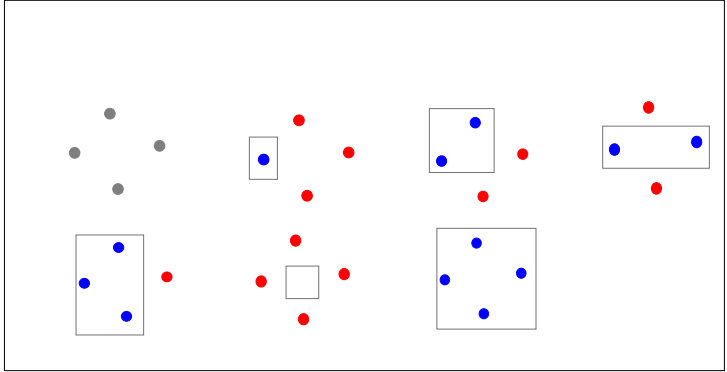
\includegraphics[width=.5\linewidth]{auto/Capture}
	\caption{Shattering of 4 points for axis aligned rectangles}
	\end{center}
	\end{figure}
  \begin{solution}
  If we take any four points randomly or on the corners of the rectangle, the adversary can label them in such a way that they will not be shatterable. So we will take a points on the edges. As we can see in the figure the points are shatterble. In case of $5$ points , our adversary can always label them in such a way that the points will never be shatterable. Therefore the VC dimension of $H^2_{rec}$ is 4.
  
  \end{solution}
  \item ~[10 poin
  ts] Generalize your argument from the previous proof
    to show that for $d$ dimensions, the VC dimension of $H^d_{rec}$
    is $2d$.
    \begin{solution}
    Using the above explanation we can see that for a 2 - dimensional of axis aligned rectangles the VC dimension was 4. This is equal to 2 times the dimensional. For an extra point there is always a point which is either inside the rectangle or is marked negative, which cannot be consistent with the axis aligned rectangles. Using the same general understanding for higher dimension we can conclude that  for d dimensions, the VC dimension of $H^d_{rec}$ is 2d.
    \end{solution}
  \end{enumerate}
  
\item In the lectures, we considered the VC dimensions of infinite
  concept classes. However, the same argument can be applied to finite
  concept classes too. In this question, we will explore this setting.

  \begin{enumerate}
  \item ~[10 points] Show that for a finite hypothesis class
    $\mathcal{C}$, its VC dimension can be at most
    $\log_2\left(|\mathcal{C}|\right)$. (Hint: You can use
    contradiction for this proof. But not necessarily!)
\begin{solution}
Considering that for a finite hypothesis class $\mathcal{C}$, its VC($\mathcal{C}$) $=$ d. As there are d points we can label them in $2^d$ ways.

The $2^d$ combinations can be in worst case classified by the size of entire hypothesis class $|\mathcal{C}|$. Therefore $2^d \leq |\mathcal{C}|$ .
Taking log on both side we get $d \leq \log_2\left(|\mathcal{C}|\right)$.
\end{solution}
  \item ~[5 points] Find an example of a class $\mathcal{C}$ of
    functions over the real interval $X = [0,1]$ such that
    $\mathcal{C}$ is an {\bf infinite} set, while its VC dimension is
    exactly one.
\begin{solution}
For a class of function over the real interval $X = [0,1]$ is a left bounded interval $[0,a)$ in it. Here we can see that the function $f(x) = +1 if 0 \leq x < a$  defines the infinite set. We know that for this the VC dimension is 1.
\end{solution}
  \item ~[5 points] Give an example of a {\bf finite} class
    $\mathcal{C}$ of functions over the same domain $X = [0,1]$ whose
    VC dimension is exactly $\log_2(|\mathcal{C}|)$.
\begin{solution}
We can see that over the same domain $X = [0,1]$ a finite class $\mathcal{C}$ is a function of Integers. Hence, we can deduce the class as $[0,1]$ where the function can either be positive for value $x=1$ or value $x=0$. There fore there are 2 functions. But only one of them is shatterable, which is VC = $\log_2 (2) = 1$. Hence VC dimension for it is exactly $\log_2(|\mathcal{C}|)$.
\end{solution}
  \end{enumerate}
  
\end{enumerate}

%%% Local Variables:
%%% mode: latex
%%% TeX-master: "hw3"
%%% End:



\end{document}
%%% Local Variables:
%%% mode: latex
%%% TeX-master: t
%%% End:
